\marginpar{VL am 06.05.19}
\section{Modelltypen und Beschreibungsformen ereignisdiskreter Systeme}

\underline{Ereignisdiskrete Systeme (DES)}

Diskreter, abzählbarer Zustandsraum ohne natürliche Ordnung der Zustände.
\begin{itemize}
	\item kein Abstandsmaß für eine eventuelle differentielle/integrale Betrachtung
	\item Analyse und Synthese meist auf Suchalgorithmen basierend (Problem: kombinatorische Explosion)
\end{itemize}

\underline{Übersicht über Modelltypen und Beschreibungsformen}\beiblatt{2-1}

\begin{figure}[H]
	\centering
	\includegraphics[page=11,scale=0.55]{material/AEH_2019.pdf}
\end{figure}

\properparagraph{Übergangsverhalten: beschreibt Zustandsübergänge}
Beispiel:
\begin{figure}[H]
	\centering
	\includegraphics[width=0.2\textwidth]{img/2019_05_06/abb1.tikz}
\end{figure}
\begin{itemize}
	\item \textcolor{green}{deterministisch}
	\item \textcolor{blue}{nicht deterministisch}
	\item \textcolor{red}{stochastisch}
\end{itemize}

\properparagraph{Zeitverhalten: beschreibt Zeitabhängigkeit der Zustandsübergänge}
\begin{figure}[H]
	\centering
	\includegraphics[width=0.6\textwidth]{img/2019_05_06/abb2.tikz}
\end{figure}
\begin{itemize}
	\item \textcolor{black}{kausal}
	\item \textcolor{green}{zeitbewertet}
	\item \textcolor{blue}{stochastische Zeitinvtervalle}
\end{itemize}

\underline{hier:}

\begin{itemize}
	\item Automaten, Petri-Netze, NCE-Systeme
	\item Formale Sprachen, Max-Plus-Algebra
\end{itemize}

\subsection{Automaten und formale Sprachen}
\begin{itemize}
	\item zu Grundlagen der theoretischen Informatik gehörig
	\item älteste DEM-Modellierung (seit 1943)
\end{itemize}

\subsubsection{Automaten}
\underline{hier:} endliche Automaten betrachtet. Def. \beiblatt{2-2}

\properparagraph{Repräsentation}
\begin{itemize}
	\item Automatentafel (Transitionstafel)
	\smash{\raisebox{-.5\dimexpr1\baselineskip+4\itemsep+2\parskip}{$\left.\rule{0pt}{.5\dimexpr2\baselineskip+3\itemsep+3\parskip}\right\}\text{(s. \beiblatt{2-2})}$}} 
	\item Automatengraph 
\end{itemize}

\underline{Beispiel: } Mealy-Automat \beiblatt{2-5}

\subsubsection{Formale Sprachen}
formales Beschreibungsmittel für DES

\properparagraph{Grundbegriffe}
\beiblatt{2-3}

\underline{Beispiel:}
\begin{equation}
	\underbrace{E}_\text{Alphabet} = \{\underbrace{e_1, e_2, e_3}_\text{Symbole}\}
\end{equation}

\begin{equation}
\text{Wörter}\left\{
\begin{aligned}
s_1 &= e_2 \\
s_2 &= e_1 e_2 \\
\end{aligned}
\right.
\end{equation}

\begin{equation}
	L_1(E) = \{s_1, s_2\} = \{e_1, e_1 e_3\} 
\end{equation}

\begin{equation}
	L_2(E) = \{ \text{Alle Wörter der Länge } n \}
\end{equation}

\begin{equation}
	L_1^{\ast}(E) = \{ \underbrace{\epsilon}_\text{leeres Wort}, e_2, e_1 e_3, e_2 e_2, e_2 e_1 e_3, e_1 e_3 e_1 e_3, \ldots \}
\end{equation}

\properparagraph{Zusammenhang mit den endlichen Automaten}
Reguläre Sprachen: \beiblatt{2-4}

es gilt: jede reguläre Sprache kann von einem endlichen Automaten repräsentiert werden.

\underline{Beispiel:} $L(E) = \{e_1^{\ast} e_2\} \qquad (E=\{e_1,\,e_2\})$

\begin{figure}[H]
	\centering
	\includegraphics[width=0.3\textwidth]{img/2019_05_06/abb3.tikz}
\end{figure}

Analog: für jeden endlichen Automaten $A$ gibt es eine spezifische reguläre Sprache $L_A$, die er akzeptiert. (s. \textit{BB AEH 2-4})

\underline{Beispiel: } Mealy-Automat auf \beiblatt{2-5}
\begin{equation}
	L_A = \{ (e_3^{\ast}(e_1 (e_2 e_3)^{\ast} e_1 e_2)^{\ast})^{\ast} \}
\end{equation}
(s. \textit{BB AEH 2-5})

\underline{in Vorlesung: } Petri-Netze als Alternative DES-Modelle fokussiert.

\includepdf[pages={12-15}]{material/AEH_2019.pdf}

\subsection{Petri-Netze}
\textsc{Karl-Adam Petri}: \textit{"Kommunikation mit Automaten"} (1926)

\underline{$\overbrace{\text{Petri-Netz}}^{\text{PN}}\text{-Darstellung}$}

\begin{itemize}
	\item \textbf{grafisch:} diputtdftdt gerichteter Graph (mit Zustandskennzeichnung)
	\item \textbf{algebraisch:} Netzmatrix $N$\footnote{Führt auf algebraische Gleichung für die Dynamik} (nur PN-Struktur) 
\end{itemize}

\subsubsection{Netztopologie}

\underline{PN-Elemente} \beiblatt{2-6}

\begin{tabularx}{0.9\linewidth}{p{2.1cm}p{0.1cm}X}
	Stellen & $\mathrel{\hat{=}}$ & Zustände \\
	Transitionen & $\mathrel{\hat{=}}$ & Ereignisse \\
	Kanten & $\mathrel{\hat{=}}$ & kausale Zusammenhänge \\
	Marken & $\mathrel{\hat{=}}$ & Kennzeichnung des aktuellen Zustands, Dynamik durch Netzparameter festgelegt \\
\end{tabularx}

\underline{Beispiel:}

\begin{subequations}
	\begin{align}
	S &= \{ s_1, s_2 \} \\
	T &= \{ t_1, t_2 \} \\
	F &= F_{pre} \cup F_{post} = \{ (s_1, t_1), (s_2,t_2) \} \cup \{(t_1, s_2), (t_2, s_1) \} \\
	K&:\; K(s_1)=1, \qquad K(s_2)=2 \\
	W&:\; W(s_1,t_1)=1, \qquad W(t_1,s_2)=2, \qquad W(s_2,t_2)=2, \qquad W(t_2,s_1)=1 \\
	M_0&:\; M_0(s_1)=1, \qquad M_0(s_2)=0
	\end{align}
\end{subequations}


für Dynamik (siehe Abschnitt~\ref{sec:netzdynamik}) Kennzeichnung von bestimmten PN-Bereichen sinnvoll \beiblatt{2-7}

\underline{Beispiel: }

\begin{figure}[H]
	\centering
	\includegraphics[width=0.3\textwidth]{img/2019_05_06/abb4.tikz}
\end{figure}

\begin{align}
	\bullet s_1 &= \{\} = \bullet s_2 \\
	s_1 \bullet &= \{t_1\} = s_2 \bullet \\
	\bullet s_3 &= \{t_3\} \\
	s_3 \bullet &= \{\} \\
	\bullet t_1 &= \{s_1,\, s_2\} \\
	t_1 \bullet &= \{s_3\}
\end{align}

\includepdf[pages={16 - 17}]{material/AEH_2019.pdf}